\documentclass[11pt,a4paper]{article}
\usepackage[utf8]{inputenc}
\usepackage{geometry}
\geometry{top=1in, bottom=1in, left=1in, right=1in}
\usepackage{amsmath, amssymb, amsfonts, bm}
\usepackage{graphicx}
\usepackage{booktabs}
\usepackage{hyperref}
\usepackage{tikz}
\usetikzlibrary{positioning, calc, arrows.meta}
\usepackage{listings}
\usepackage{color}

% Color definitions for consistent styling
\definecolor{primary}{RGB}{30, 41, 59}       % Dark Slate
\definecolor{secondary}{RGB}{14, 116, 144}   % Teal Accent
\definecolor{codebg}{RGB}{241, 245, 249}      % Light gray

\hypersetup{
    colorlinks=true,
    linkcolor=secondary,
    citecolor=secondary,
    urlcolor=secondary
}

\title{\textbf{Literature Review on Multimodal Information Retrieval:\\Learned Sparse Retrieval, Compositional Grounding, and Reasoning-Intensive Pipelines}}
\author{\textbf{Esteban Schafir} \\ FIU Research}
\date{\today}

\begin{document}

\maketitle

\begin{abstract}
This literature review provides an exhaustive and structured summary of six key research papers in the domain of Multimodal Information Retrieval (MMIR). We examine state-of-the-art approaches to bridging the gap between visual information (images, diagrams, and document layouts) and textual search capabilities. Specifically, we cover: (1) \textbf{V-SPLADE}, an inference-free sparse visual-document retriever using caption-gated token supervision; (2) \textbf{PDF-WuKong}, an end-to-end sparse sampling multimodal large language model for long PDF understanding; (3) \textbf{Grounding CLIP (GCLIP)}, a training-free compositional image-text matching framework using GPT-3.5 and Grounding DINO; (4) \textbf{Dense2Sparse (D2S)}, which converts pre-trained dense models into sparse representations using probabilistic expansion control; (5) \textbf{MLSR-IS}, a study of Multi-Modal Learned Sparse Retrieval models for image suggestion; and (6) \textbf{HIVE}, a plug-and-play LLM framework that resolves the multimodal reasoning gap at inference time. For each paper, we detail the core problem, technical methodology, mathematical formulations, concrete use cases, benchmarks, and limitations. Finally, we provide a unified comparative synthesis matrix of all reviewed works.
\end{abstract}

\newpage
\tableofcontents
\newpage

\section{Introduction}
Information retrieval (IR) has transitioned from lexical keyword matching (e.g., BM25) to semantic vector search (dense retrieval). However, the rising prevalence of multimodal content---such as academic PDFs with interleaved figures, screenshots with embedded charts, and text-image documents---has exposed massive bottlenecks in standard paradigms. 

Dense multimodal retrievers (like CLIP) project images and text into a shared embedding space but suffer from a lack of compositional generalization (failing to bind attributes to entities) and are computationally expensive at query serving time. Conversely, converting visual assets to text via optical character recognition (OCR) or visual captioning introduces high offline processing latency and text-generation costs. 

To address these challenges, two prominent paradigms have emerged in Multimodal Information Retrieval:
\begin{enumerate}
    \item \textbf{Multimodal Learned Sparse Retrieval (MMLSR):} Projecting multimodal items directly into a high-dimensional vocabulary-indexed sparse space to support exact, query-encoding-free searches via traditional inverted indexes.
    \item \textbf{Reasoning-Intensive Multimodal Pipelines:} Injecting Large Language Models (LLMs) into the retrieval loop to interpret visual layouts and synthesize compensatory queries that resolve logical reasoning gaps.
\end{enumerate}
This literature review details six seminal papers paving the path for these paradigms.

---

\section{Paper 1: Inference-Free Multimodal Learned Sparse Retrieval (V-SPLADE)}
\label{sec:v_splade}

\subsection{Core Problem and Motivation}
Visual document retrieval (VDR) requires finding relevant document page images for a text query. State-of-the-art visual document retrievers (e.g., ColPali) use late-interaction Vision-Language Models (VLMs) but require neural query encoding at query time and expensive multi-vector comparisons. While text-based learned sparse retrieval (LSR) models like SPLADE map items directly to a vocabulary to avoid query-time neural encoding, visual sparse retrieval remains underexplored.

Cho et al. (2026) identify a major bottleneck in MMLSR: the \textbf{lexical grounding problem}. Unlike text documents where input words serve as explicit anchors for vocabulary activations, visual document retrievers must infer which vocabulary dimensions to activate purely from raw pixels. As a result, standard visual sparse encoders produce noisy outputs and miss important textual terms. To solve this, they introduce \textbf{V-SPLADE}, which uses a training-only \textbf{caption-gated token supervision} signal to align visual features with discrete lexical vocabularies.

\subsection{Methodology and Mathematical Formulations}
V-SPLADE combines a visual-to-sparse document encoder with a query-token lookup table to serve queries without neural encoding.

\subsubsection{Image-Side Sparse Representation}
Let $\{h_t\}_{t=1}^L$ be the sequence of visual hidden states output by the visual encoder. The sparse document representation $w_p \in \mathbb{R}^{|V|}$ is computed by applying an LM head projection, a Rectified Linear Unit (ReLU), and max pooling over all visual tokens:
\begin{equation}
w_p[v] = \max_{t=1 \dots L} \log(1 + \text{ReLU}(\text{LMHead}(h_t)[v]))
\end{equation}
where $v$ is a vocabulary token and $|V|$ is the vocabulary size.

\subsubsection{Query-Encoding-Free Lookup}
At serving time, V-SPLADE represents a query $q$ as a weighted bag-of-words (BoW) vector $w_q \in \mathbb{R}^{|V|}$. To avoid neural query encoding, it uses a softplus-activated learned vocabulary-level lookup table:
\begin{equation}
a_v = \text{softplus}(\bm{e}_v^T \bm{u} + b)
\end{equation}
\begin{equation}
w_q[v] = m_q[v] \cdot a_v
\end{equation}
where $\bm{e}_v$ is the frozen token embedding, $\bm{u} \in \mathbb{R}^d$ and $b \in \mathbb{R}$ are learned query projection parameters, and $m_q[v] \in \{0, 1\}$ is a binary query token mask indicating the presence of term $v$ in $q$. 

\subsubsection{Caption-Gated Token Supervision}
To solve the lexical grounding problem, V-SPLADE utilizes a VLM-generated caption during training only. Let $w_p^{\text{sg}}$ and $w_c^{\text{sg}}$ be the stop-gradient sparse vectors for the page image and its offline caption, respectively. The overlap gate $o[v]$ is defined as:
\begin{equation}
o[v] = w_p^{\text{sg}}[v] \cdot w_c^{\text{sg}}[v]
\end{equation}
The gate targets $\alpha[v]$ are obtained via temperature sharpening ($\tau_{\text{cap}}$) and $L1$-normalization:
\begin{equation}
\alpha[v] = \frac{o[v]^{1/\tau_{\text{cap}}}}{\sum_{v'} o[v']^{1/\tau_{\text{cap}}}}
\end{equation}
The caption-gated token supervision loss is formulated as:
\begin{equation}
L_{\text{cap\_gated}} = -\frac{1}{B} \sum_{i=1}^B \sum_v \alpha_i[v] \log \sigma(z_{p_i}[v])
\end{equation}
where $z_p[v]$ is the image-side vocabulary logit before activation and $B$ is the batch size. 

\subsection{Concrete Use Case Example}
Suppose a user submits the text query: \texttt{"multimodal sparse retrieval"}.
\begin{enumerate}
    \item \textbf{Offline Document Indexing:} A PDF page displaying a diagram of V-SPLADE is passed directly to the V-SPLADE visual encoder. The model maps the page pixels directly to a sparse lexical vector (e.g., activating terms like \texttt{sparse} (weight 4.2), \texttt{retrieval} (weight 3.9), \texttt{multimodal} (weight 3.5), and \texttt{inverted} (weight 1.8)). It stores these weights in a standard inverted index.
    \item \textbf{Online Query Search:} When the query is typed, the system tokenizes it into \texttt{"multimodal"}, \texttt{"sparse"}, and \texttt{"retrieval"}. Instead of running a neural model to encode the query, the retriever looks up the softplus weights for these three words in the learned vocabulary table, yielding weights $\{1.5, 2.1, 2.5\}$.
    \item \textbf{Matching:} The scoring engine takes the dot product of the query weights and indexed document weights, returning the page in sub-10ms using standard inverted-index search software (like PISA).
\end{enumerate}

\subsection{Key Results, Datasets, and Limitations}
\begin{itemize}
    \item \textbf{Datasets:} Evaluated on the ViDoRe (v1, v2, v3) benchmarks, VisRAG, VisDoc OOD, and IRPAPERS.
    \item \textbf{Performance:} V-SPLADE quality variant improves average NDCG@5 by +13.8pp over the dense BiModernVBERT baseline. Under corpus scaling up to 18.7M documents, V-SPLADE retains recall much more robustly than dense retrievers.
    \item \textbf{Throughput:} Encourages 20.19 pages/sec encoding throughput on an NVIDIA H100, which is over 20x faster than traditional OCR- or captioning-based BM25 pipelines.
    \item \textbf{Limitations:} The quality of lexical grounding relies on the descriptive richness of the offline caption generator during training. Furthermore, evaluations are restricted to English-language visual documents.
\end{itemize}

---

\section{Paper 2: PDF-WuKong: Efficient Long PDF Reading with End-to-End Sparse Sampling}
\label{sec:pdf_wukong}

\subsection{Core Problem and Motivation}
Large multimodal models (MLLMs) excel at processing single-page documents but struggle with long PDFs containing interleaved text and images (such as academic papers). Feeding all document pages as high-resolution images generates thousands of visual tokens, leading to out-of-memory errors and context length issues. Conversely, pure text-based retrievers ignore crucial diagrams and mathematical equations.

Xie et al. (2026) introduce \textbf{PDF-WuKong}, an MLLM architecture designed for question-answering (QA) on long PDF documents. PDF-WuKong integrates a lightweight, query-driven \textbf{multimodal sparse sampler} that reuses the MLLM's visual encoder. By retrieving only the paragraph text blocks and image blocks (diagrams/tables) most pertinent to the query, PDF-WuKong processes documents of arbitrary length efficiently in an end-to-end manner.

\subsection{Methodology and Architecture}
The PDF-WuKong workflow operates in three main stages: document parsing, multimodal sparse sampling, and response generation.

\begin{figure}[htbp]
\centering
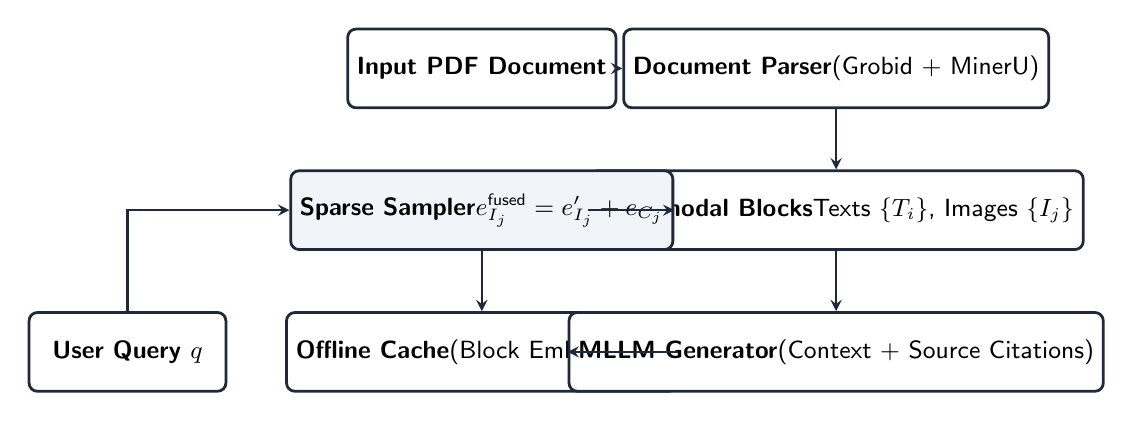
\begin{tikzpicture}[node distance=1.8cm, every node/.style={fill=white, font=\sffamily\small}]
    \tikzstyle{block} = [draw, rectangle, minimum width=2.5cm, minimum height=1cm, text centered, rounded corners=3pt, draw=primary, line width=1pt]
    \tikzstyle{data} = [draw, database, minimum width=2cm, minimum height=1cm, text centered, draw=secondary, line width=1pt]
    \tikzstyle{arrow} = [thick, ->, >=stealth, draw=primary]

    % Nodes
    \node (pdf) [block] {\textbf{Input PDF Document}};
    \node (parser) [block, right of=pdf, node distance=4.5cm] {\textbf{Document Parser}\\(Grobid + MinerU)};
    \node (blocks) [block, below of=parser, node distance=1.8cm] {\textbf{Multimodal Blocks}\\Texts $\{T_i\}$, Images $\{I_j\}$};
    \node (sampler) [block, left of=blocks, node distance=4.5cm, fill=codebg] {\textbf{Sparse Sampler}\\$e^{\text{fused}}_{I_j} = e'_{I_j} + e_{C_j}$};
    \node (cache) [block, below of=sampler, node distance=1.8cm] {\textbf{Offline Cache}\\(Block Embeddings)};
    \node (query) [block, left of=cache, node distance=4.5cm] {\textbf{User Query $q$}};
    \node (mllm) [block, below of=blocks, node distance=1.8cm] {\textbf{MLLM Generator}\\(Context + Source Citations)};

    % Arrows
    \draw [arrow] (pdf) -- (parser);
    \draw [arrow] (parser) -- (blocks);
    \draw [arrow] (blocks) -- (sampler);
    \draw [arrow] (sampler) -- (cache);
    \draw [arrow] (query) |- (sampler);
    \draw [arrow] (cache) -- (mllm);
    \draw [arrow] (blocks) -- (mllm);
\end{tikzpicture}
\caption{The Architecture and Data Flow of PDF-WuKong.}
\label{fig:pdf_wukong}
\end{figure}

\subsubsection{Document Parsing and Representation}
PDF-WuKong parses a document $D$ into structured text blocks $\{T_1 \dots T_n\}$ and image blocks $\{I_1 \dots I_m\}$ (each associated with its caption $C_j$) using a hybrid pipeline of Grobid and MinerU.

\subsubsection{Multimodal Sparse Sampling}
\begin{itemize}
    \item \textbf{Text Embedding:} Each text block $T_i$ is embedded using a lightweight text encoder $E_T(\cdot)$ to obtain $e_{T_i} \in \mathbb{R}^{d_T}$ (specifically, BGE-M3).
    \item \textbf{Image Embedding:} For each image block $I_j$, visual sequence features $e_{I_j}$ are extracted using the MLLM's visual encoder $E_V(\cdot)$. These features are mean-pooled and projected to the text embedding space via a learned MLP head $\text{MLP}_{\text{proj}}$:
    \begin{equation}
    e'_{I_j} = \text{MLP}_{\text{proj}}(\text{MeanPool}(e_{I_j})) \in \mathbb{R}^{d_T}
    \end{equation}
    If the image has an associated caption $C_j$, the caption text is encoded as $e_{C_j} = E_T(C_j)$, and the final representation is fused via element-wise addition:
    \begin{equation}
    e^{\text{fused}}_{I_j} = e'_{I_j} + e_{C_j}
    \end{equation}
\end{itemize}

\subsubsection{Query-driven Retrieval and Generation}
Given query $q$, the query embedding is $e_q = E_T(q)$. Cosine similarities are computed to select the top-$K$ blocks. 
For generation, the original visual sequence embeddings $e_{I_j}$ of selected images are projected into the LLM space using the native connection module $\text{MLP}_{\text{conn}}$, preserving fine-grained details:
\begin{equation}
\hat{e}_{I_j} = \text{MLP}_{\text{conn}}(e_{I_j})
\end{equation}
The MLLM receives the query $q$, raw paragraph text $T_i$, captions $C_j$, and visual context tokens $\hat{e}_{I_j}$ to synthesize the final answer.

\subsection{Concrete Use Case Example}
A researcher is reading a 60-page PDF paper and asks: \texttt{"What is the performance of the COP algorithm in Figure 4?"}
\begin{enumerate}
    \item \textbf{Offline Phase:} PDF-WuKong parses the document, extracting 150 text blocks and 8 figures. It embeds and caches all of them offline.
    \item \textbf{Online Retrieval:} The text query is embedded. The sparse sampler computes similarity, identifying that \texttt{"Figure 4"} (an image block) and its caption \texttt{"Comparison of COP pruning against standard baselines"} share high cosine similarity with the query. They are retrieved as evidence blocks.
    \item \textbf{Generation:} The LLM receives the visual patch tokens of Figure 4 and the text of paragraph 32. It generates: \texttt{"According to Figure 4, the COP algorithm (block index [Image 4]) achieves a 93\% accuracy, outperforming the baseline by 5.2\% as explained in block [Para 32]."}
\end{enumerate}

\subsection{Key Results, Datasets, and Limitations}
\begin{itemize}
    \item \textbf{Datasets:} Tested on the newly constructed PaperPDF dataset (1.1M bilingual training QA pairs, 10k evaluation QA pairs), DUDE, and MM-NIAH.
    \item \textbf{Performance:} PDF-WuKong surpasses leading open-source models and proprietary document assistants on PaperPDF by an average of +8.6\% F1 score. It maintains high accuracy even as document context scales to 64K tokens.
    \item \textbf{Limitations:} Relies on layout parsers (Grobid/MinerU); errors in reading order extraction or layout segmentation propagate directly to the sparse sampler, causing relevant blocks to be missed.
\end{itemize}

---

\section{Paper 3: Compositional Image-Text Matching and Retrieval by Grounding Entities (GCLIP)}
\label{sec:gclip}

\subsection{Core Problem and Motivation}
Foundational Vision-Language Models (VLMs) like CLIP embed entire images and text captions globally. However, they lack a deep understanding of \textbf{compositional syntax} (the relation between subjects, predicates, and objects). CLIP behaves like a bag-of-words model, often matching captions containing specific terms with incorrect images due to dataset biases and co-occurrence priors. 

For instance, CLIP struggles to distinguish between \texttt{"A man is holding a sign"} and \texttt{"A man is holding glasses"} because the dominant tokens (\texttt{"man"}, \texttt{"holding"}) are present in both, and the model lacks a mechanism to verify if the subject is bound to the correct object. Vongala et al. (2025) introduce \textbf{Grounding CLIP (GCLIP)}, a training-free, zero-shot framework that dynamically refines CLIP's global image embedding using noun phrase localization.

\subsection{Methodology and Pipeline}
GCLIP adjusts the global CLIP image embedding using an open-vocabulary detector.

\subsubsection{Text Decomposition}
GCLIP prompts GPT-3.5-turbo to decompose the input caption $T$ into its core entities $O = \{o_1 \dots o_n\}$, their attributes, and relational structures, generating short descriptions for each.

\subsubsection{Open-Vocabulary Grounding}
Using the parsed entity names, GCLIP utilizes \textbf{Grounding DINO} to localize and extract bounding box coordinates for each entity within the image:
\begin{equation}
B_i = \text{GroundingDINO}(I, o_i)
\end{equation}
where $B_i$ represents the bounding box coordinates for entity $o_i$ in image $I$.

\subsubsection{Dynamic Embedding Refinement}
The image regions corresponding to the bounding boxes are cropped and passed through the CLIP vision encoder to obtain local embeddings $e_{o_i}$. GCLIP refines the global image embedding $I$ to create a compositionally grounded embedding $I_c$ by taking a weighted sum of the global embedding and the localized sub-image embeddings:
\begin{equation}
I_c = I + \sum_{i=1}^n \beta_i \cdot e_{o_i}
\end{equation}
where $\beta_i$ is a dynamic weight factor. The similarity score is computed as:
\begin{equation}
\text{Score}(I, T) = \cos(I_c, T_{\text{global}})
\end{equation}

\subsection{Concrete Use Case Example}
An image retrieval system is queried with the caption: \texttt{"A cat sitting on top of a laptop"}.
The candidate database contains two similar images: Image A (a cat sitting next to a closed laptop) and Image B (a cat sitting directly on top of an open laptop).
\begin{enumerate}
    \item \textbf{Text Parsing:} GPT-3.5 extracts entities: \texttt{"cat"}, \texttt{"laptop"}, and the relation \texttt{"cat on top of laptop"}.
    \item \textbf{Entity Grounding:} Grounding DINO detects the cat and laptop bounding boxes in both images.
    \item \textbf{Refinement:} GCLIP computes local embeddings for the cropped cat and laptop regions. For Image B, the localized spatial relation matches the syntax. The adjusted embedding $I_c$ for Image B aligns with the text embedding of the query, resulting in a higher cosine score than Image A.
\end{enumerate}

\subsection{Key Results, Datasets, and Limitations}
\begin{itemize}
    \item \textbf{Datasets:} Evaluated on Flickr30K, MS-COCO, ComVG, and SVO Probes.
    \item \textbf{Performance:} GCLIP improves the state-of-the-art zero-shot Recall@1 by +12\% on Flickr30K and +0.4\% on MS-COCO.
    \item \textbf{Limitations:} It is a multi-stage, pipeline-based approach that relies on LLM API calls and object detectors at query time. This introduces significant latency, making it unsuitable for low-latency, large-scale search scenarios unless candidates are pre-cached.
\end{itemize}

---

\section{Paper 4: Multimodal Learned Sparse Retrieval with Probabilistic Expansion Control (D2S)}
\label{sec:d2s}

\subsection{Core Problem and Motivation}
Training Multimodal Learned Sparse Retrieval (MMLSR) models from scratch (such as LexLIP and STAIR) is computationally expensive, requiring multi-step training on millions or billions of image-text pairs. An alternative is to project pre-trained dense embeddings (e.g., BLIP or ALBEF) into a sparse vocabulary space. 

However, Nguyen et al. (2024) identify that naively training a projection head on top of dense models causes:
\begin{enumerate}
    \item \textbf{Dimension Co-activation:} Text and image sparse vectors over-activate the same set of vocabulary terms, collapsing the high-dimensional sparse space into a sub-dense space. This leads to long posting lists and slow search speeds.
    \item \textbf{Semantic Deviation:} The sparse projection activates irrelevant words (semantic hallucinations) that do not match the image content, reducing search accuracy and human interpretability.
\end{enumerate}
To solve this, they propose \textbf{Dense2Sparse (D2S)} equipped with \textbf{Probabilistic Expansion Control (PEC)}.

\subsection{Methodology and Formulations}
D2S projects dense vectors to a sparse vocabulary space while using Bernoulli gates to regulate term expansion during training.

\subsubsection{Sparse Projection Head}
Let $z_C = f_{\phi}^C(x_C) \in \mathbb{R}^d$ and $z_I = f_{\theta}^I(x_I) \in \mathbb{R}^d$ be the dense embeddings from frozen text and image encoders. The sparse projection head $g_{\psi}(\cdot)$ computes:
\begin{equation}
z_1 = W_1 z
\end{equation}
\begin{equation}
z_2 = \frac{z_1 - E[z_1]}{\sqrt{\text{Var}[z_1] + \epsilon}} \cdot \gamma + \beta
\end{equation}
\begin{equation}
s = W_2 z_2
\end{equation}
\begin{equation}
\text{D2S}(z) = \log_e(1 + \max(0, s)) \in \mathbb{R}^{|V|}_{\geq 0}
\end{equation}
where $W_1 \in \mathbb{R}^{\omega \times d}$, $W_2 \in \mathbb{R}^{|V| \times \omega}$, and $\gamma, \beta$ are learnable normalization parameters.

\subsubsection{Probabilistic Expansion Control}
To prevent co-activation, D2S regulates term expansions during training using Bernoulli gates. Let $E_C \sim \text{Ber}(p_c)$ be a caption-level gate, and $E^v_i \sim \text{Ber}(p_v)$ be a word-level gate. For document sparse vector $s_C$, the gated vector $s_C^{\text{PEC}}$ is defined as:
\begin{equation}
s_C^{\text{PEC}}[i, k] = \begin{cases}
s_C[i, k] \cdot E_C \cdot E^v_k & \text{if } v_k \notin x_C \\
s_C[i, k] \cdot E^v_k & \text{if } v_k \in x_C
\end{cases}
\end{equation}
During training, $p_c$ is initially set to 0 (no term expansion, forcing the model to activate only words present in the text description $x_C$). As training progresses, $p_c$ and $p_v$ are gradually scaled up using a scheduler $f_{\text{incr}}(p)$, allowing the model to learn semantic expansions (synonyms) without losing grounding.

\subsection{Concrete Use Case Example}
An image of a \texttt{"golden retriever chasing a tennis ball"} is indexed.
\begin{enumerate}
    \item \textbf{Without PEC:} The projection head over-activates generic words like \texttt{"photo"}, \texttt{"picture"}, \texttt{"the"}, and unrelated items like \texttt{"cat"} or \texttt{"frisbee"}. This creates a dense, noisy index representation.
    \item \textbf{With PEC:} The Bernoulli gates suppress expansions during early training epochs, forcing the projection head to align with exact tokens: \texttt{dog}, \texttt{golden}, \texttt{ball}, \texttt{tennis}. During later epochs, it expands to relevant terms: \texttt{retriever}, \texttt{fetch}, \texttt{grass}. The resulting index is highly sparse and accurate.
\end{enumerate}

\subsection{Key Results, Datasets, and Limitations}
\begin{itemize}
    \item \textbf{Datasets:} MSCOCO and Flickr30k.
    \item \textbf{Performance:} D2S achieves competitive retrieval accuracy compared to models trained from scratch (like LexLIP) while requiring a fraction of the training time and GPU memory.
    \item \textbf{Limitations:} The model relies on the representation quality of the frozen dense encoders. If the base model fails to capture a visual concept, the sparse projection cannot recover it.
\end{itemize}

---

\section{Paper 5: Multimodal Learned Sparse Retrieval for Image Suggestion (MLSR-IS)}
\label{sec:mlsr_is}

\subsection{Core Problem and Motivation}
The image suggestion task aims to retrieve relevant images for a given text query (e.g., finding illustrations for an article). Standard sparse retrievers are text-only. Applying sparse retrieval to images requires mapping visual features into a text vocabulary space.

Nguyen, Hendriksen, and Yates (2023) evaluate different configurations of Multimodal Learned Sparse Retrieval (MLSR) models. They compare Multi-Layer Perceptron (MLP) and Masked Language Model (MLM) projection heads, and analyze the performance impact of using image content alone versus enriching images with their captions.

\subsection{Methodology and Architectures}
The authors define a bi-encoder architecture and evaluate three document representation configurations:

\begin{figure}[htbp]
\centering
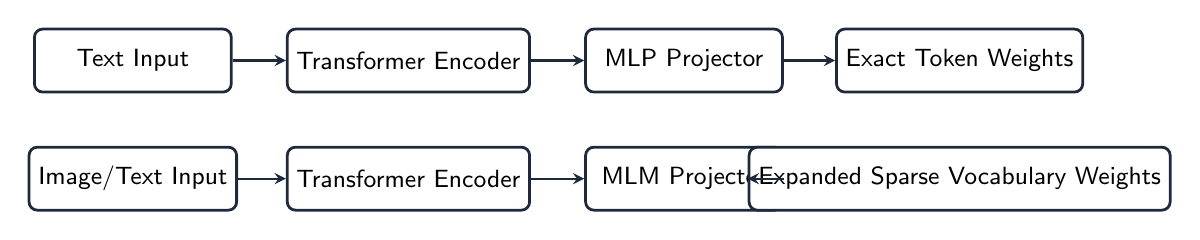
\begin{tikzpicture}[node distance=1.5cm, every node/.style={fill=white, font=\sffamily\small}]
    \tikzstyle{block} = [draw, rectangle, minimum width=2.5cm, minimum height=0.8cm, text centered, rounded corners=3pt, draw=primary, line width=1pt]
    \tikzstyle{arrow} = [thick, ->, >=stealth, draw=primary]

    % MLP Encoder Flow
    \node (text1) [block] {Text Input};
    \node (trans1) [block, right of=text1, node distance=3.5cm] {Transformer Encoder};
    \node (mlp) [block, right of=trans1, node distance=3.5cm] {MLP Projector};
    \node (out1) [block, right of=mlp, node distance=3.5cm] {Exact Token Weights};

    % MLM Encoder Flow
    \node (vis1) [block, below of=text1, node distance=1.5cm] {Image/Text Input};
    \node (trans2) [block, right of=vis1, node distance=3.5cm] {Transformer Encoder};
    \node (mlm) [block, right of=trans2, node distance=3.5cm] {MLM Projector};
    \node (out2) [block, right of=mlm, node distance=3.5cm] {Expanded Sparse Vocabulary Weights};

    % Arrows
    \draw [arrow] (text1) -- (trans1);
    \draw [arrow] (trans1) -- (mlp);
    \draw [arrow] (mlp) -- (out1);
    \draw [arrow] (vis1) -- (trans2);
    \draw [arrow] (trans2) -- (mlm);
    \draw [arrow] (mlm) -- (out2);
\end{tikzpicture}
\caption{Comparison of MLP and MLM Sparse Projections.}
\label{fig:mlp_mlm}
\end{figure}

\begin{enumerate}
    \item \textbf{Image-Only ($M_{T \to I}$):} The document representation is constructed from the image content only using an MLM projection head.
    \item \textbf{Caption-Only ($M_{T \to T}$):} The document representation is constructed from the textual caption only.
    \item \textbf{Hybrid ($M_{T \to T+I}$):} The document representation is constructed from both the image content and the caption text.
\end{enumerate}

\subsubsection{MLP vs. MLM Projection Heads}
\begin{itemize}
    \item \textbf{MLP Head:} Takes contextualized token embeddings $h_j$ and projects each to a weight $w(t)$:
    \begin{equation}
    w[t] = \sum_{j=1}^L \log(1 + \text{ReLU}(h_j W + b))
    \end{equation}
    Because it requires input tokens, it can only be applied to text inputs and does not support term expansion.
    \item \textbf{MLM Head:} Projects a single pooled document embedding $h_0$ directly to the entire vocabulary space:
    \begin{equation}
    w[t] = \text{ReLU}(h_0^T e_t + b_t)
    \end{equation}
    This head can process both image and text inputs and supports vocabulary-wide term expansions.
\end{itemize}

\subsection{Concrete Use Case Example}
An editor is writing an article about \texttt{"renewable solar energy systems"} and wants the system to suggest relevant images.
\begin{enumerate}
    \item \textbf{Image-Only Search ($M_{T \to I}$):} An image of solar panels is indexed using visual tokens. Without textual context, the model fails to capture the technical concept of \texttt{"renewable energy"}, returning lower matching scores.
    \item \textbf{Hybrid Search ($M_{T \to T+I}$):} The image is indexed alongside its caption: \texttt{"photovoltaic solar panels installed on a residential rooftop"}. The MLM head maps the panel image features and caption text to terms like \texttt{solar}, \texttt{photovoltaic}, and expands them to \texttt{renewable}, \texttt{clean}, \texttt{energy}. The query matches successfully.
\end{enumerate}

\subsection{Key Results and Limitations}
\begin{itemize}
    \item \textbf{Findings:} Evaluated on TREC benchmarks, the study shows that retrieval using image content alone ($M_{T \to I}$) is challenging. Integrating textual captions ($M_{T \to T+I}$) improves retrieval performance significantly, highlighting the importance of textual context in visual retrieval.
    \item \textbf{Limitations:} The model requires high-quality image captions. In domains where captions are unavailable or noisy, retrieval performance degrades.
\end{itemize}

---

\section{Paper 6: HIVE: Hypothesis-driven Iterative Visual Evidence Retrieval}
\label{sec:hive}

\subsection{Core Problem and Motivation}
Standard multimodal retrievers underperform on reasoning-intensive queries where images (diagrams, charts, or chemical structures) must be integrated with text to identify relevant documents. For instance, on the MM-BRIGHT benchmark, state-of-the-art multimodal retrievers perform worse than text-only retrievers. This is because standard models embed images and text jointly but lack the logical capacity to reason about what visual content implies for document relevance.

Abdalla et al. (2026) introduce \textbf{HIVE} (Hypothesis-driven Iterative Visual Evidence Retrieval), a plug-and-play framework that injects visual-textual reasoning into a retriever using LLMs. HIVE operates entirely at inference time and requires no model retraining, making it compatible with any base retriever.

\subsection{Methodology and Architecture}
HIVE implements a four-stage pipeline:

\begin{figure}[htbp]
\centering
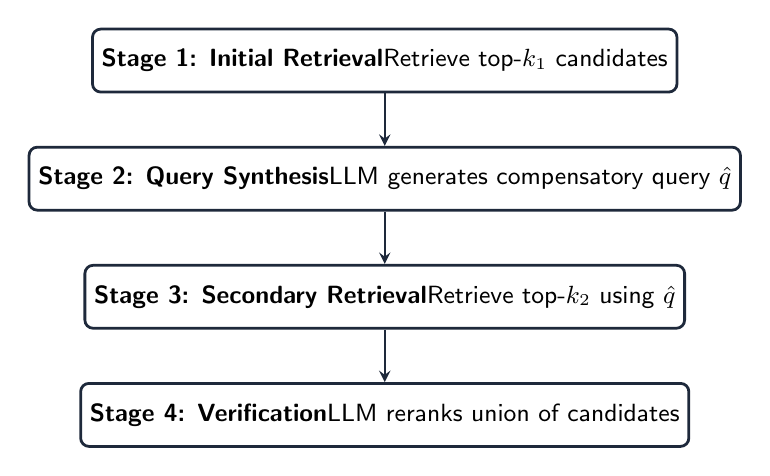
\begin{tikzpicture}[node distance=1.5cm, every node/.style={fill=white, font=\sffamily\small}]
    \tikzstyle{block} = [draw, rectangle, minimum width=3cm, minimum height=0.8cm, text centered, rounded corners=3pt, draw=primary, line width=1pt]
    \tikzstyle{arrow} = [thick, ->, >=stealth, draw=primary]

    % HIVE Stages
    \node (s1) [block] {\textbf{Stage 1: Initial Retrieval}\\Retrieve top-$k_1$ candidates};
    \node (s2) [block, below of=s1, node distance=1.5cm] {\textbf{Stage 2: Query Synthesis}\\LLM generates compensatory query $\hat{q}$};
    \node (s3) [block, below of=s2, node distance=1.5cm] {\textbf{Stage 3: Secondary Retrieval}\\Retrieve top-$k_2$ using $\hat{q}$};
    \node (s4) [block, below of=s3, node distance=1.5cm] {\textbf{Stage 4: Verification}\\LLM reranks union of candidates};

    % Arrows
    \draw [arrow] (s1) -- (s2);
    \draw [arrow] (s2) -- (s3);
    \draw [arrow] (s3) -- (s4);
\end{tikzpicture}
\caption{The Four-Stage HIVE Pipeline.}
\label{fig:hive_pipeline}
\end{figure}

\begin{enumerate}
    \item \textbf{Initial Retrieval:} A base retriever finds the top-$k_1$ candidate documents using the original text query $q_t$ and the image description $\delta(q_v)$:
    \begin{equation}
    D^{(1)} = \text{Retriever}(q_t, \delta(q_v), C, k_1)
    \end{equation}
    \item \textbf{Compensatory Query Synthesis:} An LLM compares the query image description $\delta(q_v)$ with the retrieved candidate documents $D^{(1)}$. It identifies visual and logical concepts that are missing from the initial candidates and generates a targeted compensatory query $\hat{q}$:
    \begin{equation}
    \hat{q} = \text{LLM}(\text{HypothesisPrompt}(q_t, \delta(q_v), D^{(1)}))
    \end{equation}
    \item \textbf{Secondary Retrieval:} The retriever performs a second pass using the compensatory query $\hat{q}$ to retrieve a broader candidate set:
    \begin{equation}
    D^{(2)} = \text{Retriever}(\hat{q}, q_v, C, k_2) \quad (k_2 \gg k_1)
    \end{equation}
    The candidate pool is updated to the union of both rounds: $U = D^{(1)} \cup D^{(2)}$.
    \item \textbf{Verification and Reranking:} The LLM re-evaluates the union set $U$ against the original query $(q_t, \delta(q_v))$, scoring and reranking the documents step-by-step:
    \begin{equation}
    \text{Score}(d_i) = \begin{cases}
    S_{\text{max}} - \text{rank}_i & \text{if } d_i \in D^{\text{ranked}} \\
    S_{\text{base}} - \text{offset}_i & \text{otherwise}
    \end{cases}
    \end{equation}
\end{enumerate}

\subsection{Concrete Use Case Example}
A user uploads a circuit diagram showing an open switch and asks: \texttt{"Why is my LED not lighting up?"}
\begin{enumerate}
    \item \textbf{Initial Retrieval:} The retriever searches for \texttt{"LED not lighting up"}. It retrieves documents discussing dead batteries and burnt-out resistors ($D^{(1)}$).
    \item \textbf{Compensatory Query Synthesis:} The LLM analyzes the image description (which details the open switch) and compares it with $D^{(1)}$. It notes: \texttt{"The retrieved documents ignore the state of the switch shown in the diagram."} It generates the compensatory query $\hat{q}$: \texttt{"open switch loop circuit current flow LED"}.
    \item \textbf{Secondary Retrieval:} The system retrieves documents discussing how open switches break circuit continuity.
    \item \textbf{Reranking:} The LLM evaluates the candidates and places the document explaining switch-induced open circuits at the top of the results.
\end{enumerate}

\subsection{Key Results and Limitations}
\begin{itemize}
    \item \textbf{Datasets:} Evaluated on MM-BRIGHT, spanning 2,803 queries across 29 technical domains.
    \item \textbf{Performance:} HIVE achieves an aggregated nDCG@10 of 41.7, outperforming the best multimodal baseline (Nomic-Vision: 27.6) by +14.1 points and the best text-only model by +9.5 points.
    \item \textbf{Limitations:} The multi-stage verification pipeline requires multiple LLM calls per query, introducing API latency and computational cost at inference time.
\end{itemize}

---

\section{Comparative Synthesis Matrix}
\label{sec:comparative_table}

The following table summarizes the architectural profiles, serving paradigms, modalities, benchmarks, and limitations of the reviewed models.

\begin{table}[htbp]
\centering
\small
\resizebox{\textwidth}{!}{
\begin{tabular}{lllllll}
\toprule
\textbf{Model / Paper} & \textbf{Architecture} & \textbf{Serving Paradigm} & \textbf{Training Type} & \textbf{Modalities} & \textbf{Primary Benchmarks} & \textbf{Primary Limitation} \\
\midrule
\textbf{V-SPLADE} & Sparse Encoder + & Query-encoding-free & Frozen backbone + & Image, & ViDoRe, VisRAG, & Relies on offline captions \\
(Cho et al.) & Token Lookup Table & Lexical Matching & Gated training & Text & VisDoc, IRPAPERS & during training \\
\midrule
\textbf{PDF-WuKong} & MLLM + Multi- & Dense Vector & End-to-end joint & Text, & PaperPDF, DUDE, & Parsing errors cascade \\
(Xie et al.) & modal Sampler & Similarity Retrieval & contrastive & Image & MM-NIAH & to the sampler \\
\midrule
\textbf{GCLIP} & Contrastive VLM + & Crop-level CLIP & Training-free & Image, & Flickr30K, MS-COCO, & High query-time latency \\
(Vongala et al.) & Grounding DINO & Refinement & Zero-shot & Text & ComVG, SVO Probes & from object detection \\
\midrule
\textbf{D2S (PEC)} & Frozen bi-encoder & Vocabulary projection & Frozen encoders + & Image, & Flickr30K, & Dependent on base model \\
(Nguyen et al.) & + Projection Head & Sparse Retrieval & Bernoulli gating & Text & MS-COCO & representation quality \\
\midrule
\textbf{MLSR-IS} & Sparse Bi-encoder & MLM/MLP Vocabulary & Contrastive & Image, & TREC Image & Requires high-quality \\
(Nguyen et al.) & (MLP or MLM) & Sparse Matching & pre-training & Text & Suggestion & document captions \\
\midrule
\textbf{HIVE} & Base Retriever + & Multi-stage LLM & Training-free & Image, & MM-BRIGHT & Multiple LLM calls \\
(Abdalla et al.) & LLM pipeline & Reasoning \& Reranking & Inference-only & Text & & introduce latency/cost \\
\bottomrule
\end{tabular}
}
\caption{Comparative Synthesis of Multimodal Information Retrieval Models.}
\label{tab:comparative_matrix}
\end{table}

---

\section{Conclusion and Future Work}
The reviewed literature demonstrates a clear path toward efficient and reasoning-capable Multimodal Information Retrieval. While models like V-SPLADE and D2S focus on reducing query-time latency and indexing costs via sparse representations, architectures like PDF-WuKong and frameworks like HIVE focus on resolving complex reasoning gaps for long documents and technical queries. 

Future research in this domain lies in combining these strengths: deploying training-free sparse projection layers (D2S) inside structured document samplers (PDF-WuKong) to enable low-latency, reasoning-aware visual searches at scale.

\end{document}
